\documentclass{article}

% Language setting
% Replace `english' with e.g. `spanish' to change the document language
\usepackage[german]{babel}
\usepackage{xcolor}

% Set page size and margins
% Replace `letterpaper' with `a4paper' for UK/EU standard size
\usepackage[letterpaper,top=2cm,bottom=2cm,left=3cm,right=3cm,marginparwidth=1.75cm]{geometry}

% Useful packages
\usepackage{amsmath}
\usepackage{graphicx}
\usepackage[colorlinks=true, allcolors=blue]{hyperref}
\usepackage{float}
\usepackage{multicol}
\usepackage{xcolor}



\setlength{\columnseprule}{0.5pt}
\def\columnseprulecolor{\color{blue}}



\title{}
\author{Asha Schwegler}

\begin{document}
\maketitle
\tableofcontents
\newpage



\begin{figure}[H]
\centering
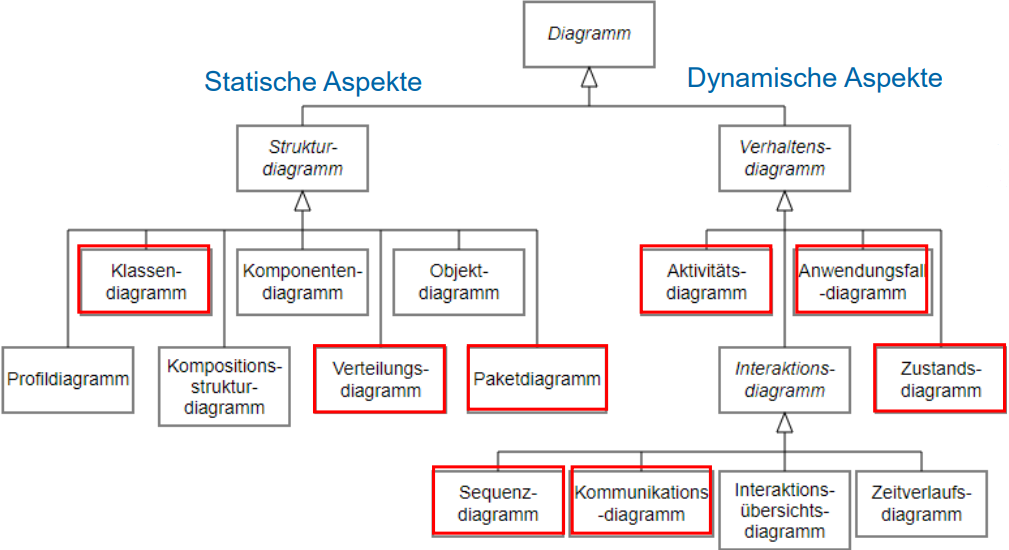
\includegraphics[width=0.3\textwidth]{Resources/Images/UML_Diagramme.png}
\caption{\label{fig:Guetereinteilung}Guetereinteilung.}
\end{figure}


\begin{table} [H]

\begin{tabular}{l}

\colorbox{pink!30}{\textbf{Massnahmen mit dem Fokus " Interaktion"} }

\\\hline
- Direkt-Mail\\
- Events\\
- Servicenummern\\
- Gewinnspiele\\
- Produktmuster\\
\hline
\colorbox{pink!30}{\textbf{Massnahmen mit dem Fokus " Zufriedenheit"}}\\
\hline
- Kundenclubs\\
- Kundenzeitschriften\\
- Beschwerdemanagement\\
\hline
\colorbox{pink!30}{\textbf{Massnahmen mit dem Fokus " Wechselbarriere"}}\\
\hline
- Rabatt- und Bonussysteme\\
- Prisdifferenzierung\\
- Kundenkarten\\
\end{tabular}
\end{table}